\selectlanguage{spanish}
\section*{Introducción}

En este artículo de final de año vamos a dar cierre al curso de Octave
que os hemos dado a lo largo de este primer volumen de la revista con
una serie de problemas. Espero leáis los problemas y antes de mirar la solución os déis un tiempo
para hacerlo por vosotros mismos. ¡Es maravilloso encontrar la solución
por uno mismo!

Durante el año hemos dado unas nociones básicas de \emph{Octave} y
puedes aumentar los conocimientos usando, por ejemplo, el siguiente
tutorial
\url{http://en.wikibooks.org/wiki/Octave_Programming_Tutorial}.

Esperamos haberte hecho mas fácil y divertido el aprendizaje de un lenguaje de programación.

\section{Esperanza de vida de Ángola}
 
Según la organización mundial de la salud la definición de esperanza
de vida es como sigue: años que un recién nacido puede esperar vivir
si los patrones de mortalidad por edades imperantes en el momento de
su nacimiento siguieran siendo los mismos a lo largo de toda su
vida. Hacer un cálculo de esta cantidades es muy complicado y se tiene
en cuenta factores como por ejemplo la medicina, la higiene, las
guerras, etc.

Lo que os proponemos es lo siguiente: dado la esperanza de vida de
Ángola proporcionada por el banco mundial de datos
(\url{http://datos.bancomundial.org/}) que proporciona datos desde 1980 a
2012, os sugerimos resolváis el siguiente desafío:

\begin{mybox}
  \begin{center}\textcolor{blue}{DESAFIO VIDA}\end{center}
  ¿En qué año tiene previsto el pueblo angolano tener una
  esperana de vida de 80 años?%\vspace{1.5cm}
\end{mybox}


\vspace{1cm} 
\textcolor{blue}{\Large Nuestra Solución}\\ 
Hemos coleccionado los datos en el archivo \emph{Hopelife.csv}. Los vamos a cargar a \emph{Octave} y vamos a echarle un vistazo a estos. El código lo podrás visualizar en la
sección de \textbf{códigos} de la revista en \url{www.revistasolucoes.com}.
\begin{table}
\begin{center}
\begin{tabular}{cc}
\scalebox{0.45}{% Title: glps_renderer figure
% Creator: GL2PS 1.3.8, (C) 1999-2012 C. Geuzaine
% For: Octave
% CreationDate: Thu Nov 13 08:58:54 2014
\setlength{\unitlength}{1pt}
\begin{picture}(0,0)
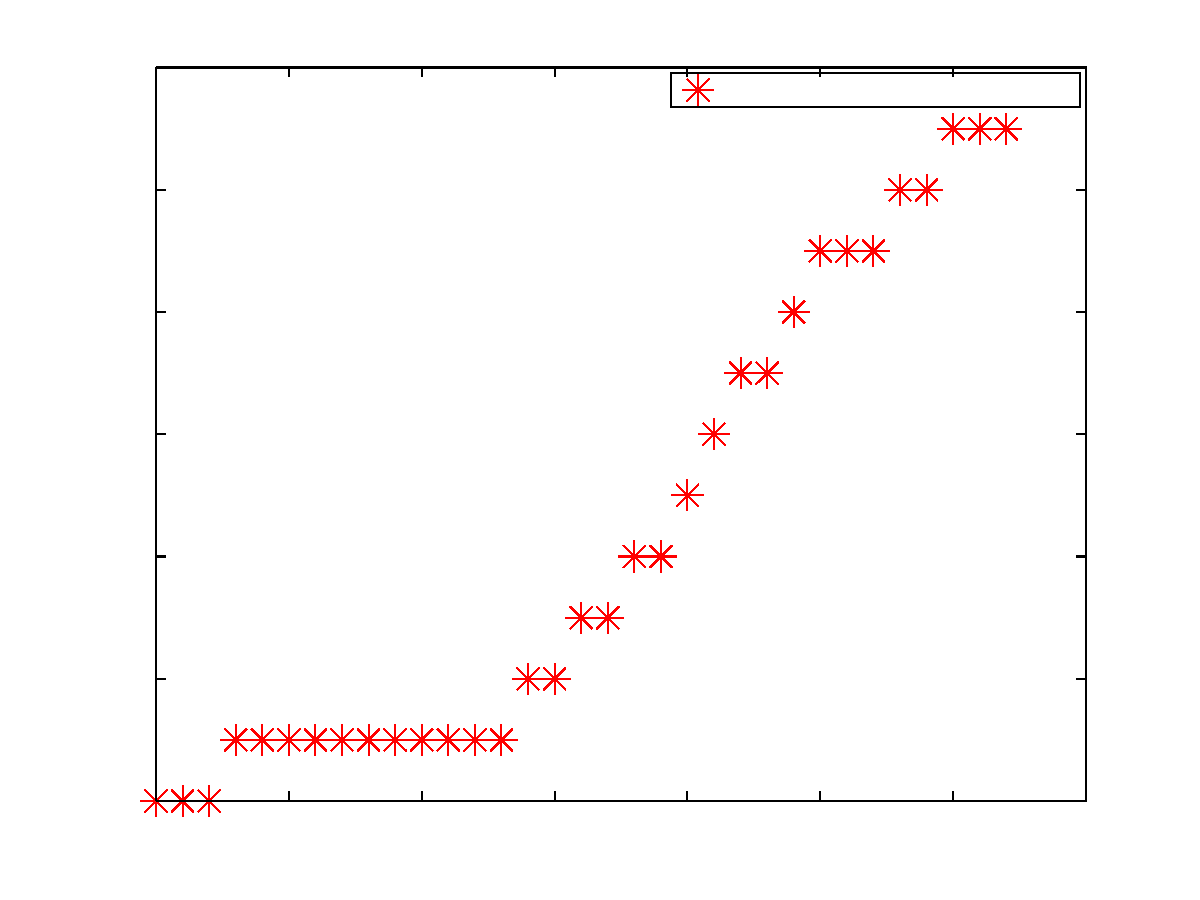
\includegraphics{DatosPuros-inc}
\end{picture}%
\begin{picture}(576,432)(0,0)
\fontsize{10}{0}
\selectfont\put(74.8806,42.519){\makebox(0,0)[t]{\textcolor[rgb]{0,0,0}{{1980}}}}
\fontsize{10}{0}
\selectfont\put(138.652,42.519){\makebox(0,0)[t]{\textcolor[rgb]{0,0,0}{{1985}}}}
\fontsize{10}{0}
\selectfont\put(202.423,42.519){\makebox(0,0)[t]{\textcolor[rgb]{0,0,0}{{1990}}}}
\fontsize{10}{0}
\selectfont\put(266.194,42.519){\makebox(0,0)[t]{\textcolor[rgb]{0,0,0}{{1995}}}}
\fontsize{10}{0}
\selectfont\put(329.966,42.519){\makebox(0,0)[t]{\textcolor[rgb]{0,0,0}{{2000}}}}
\fontsize{10}{0}
\selectfont\put(393.737,42.519){\makebox(0,0)[t]{\textcolor[rgb]{0,0,0}{{2005}}}}
\fontsize{10}{0}
\selectfont\put(457.51,42.519){\makebox(0,0)[t]{\textcolor[rgb]{0,0,0}{{2010}}}}
\fontsize{10}{0}
\selectfont\put(521.281,42.519){\makebox(0,0)[t]{\textcolor[rgb]{0,0,0}{{2015}}}}
\fontsize{10}{0}
\selectfont\put(69.8774,47.5201){\makebox(0,0)[r]{\textcolor[rgb]{0,0,0}{{40}}}}
\fontsize{10}{0}
\selectfont\put(69.8774,106.2){\makebox(0,0)[r]{\textcolor[rgb]{0,0,0}{{42}}}}
\fontsize{10}{0}
\selectfont\put(69.8774,164.88){\makebox(0,0)[r]{\textcolor[rgb]{0,0,0}{{44}}}}
\fontsize{10}{0}
\selectfont\put(69.8774,223.56){\makebox(0,0)[r]{\textcolor[rgb]{0,0,0}{{46}}}}
\fontsize{10}{0}
\selectfont\put(69.8774,282.24){\makebox(0,0)[r]{\textcolor[rgb]{0,0,0}{{48}}}}
\fontsize{10}{0}
\selectfont\put(69.8774,340.92){\makebox(0,0)[r]{\textcolor[rgb]{0,0,0}{{50}}}}
\fontsize{10}{0}
\selectfont\put(69.8774,399.6){\makebox(0,0)[r]{\textcolor[rgb]{0,0,0}{{52}}}}
\fontsize{10}{0}
\selectfont\put(298.081,29.5189){\makebox(0,0)[t]{\textcolor[rgb]{0,0,0}{{años}}}}
\fontsize{10}{0}
\selectfont\put(53.877,223.56){\rotatebox{90}{\makebox(0,0)[b]{\textcolor[rgb]{0,0,0}{{esperanza de vida}}}}}
\fontsize{10}{0}
\selectfont\put(298.081,409.6){\makebox(0,0)[b]{\textcolor[rgb]{0,0,0}{{Evolución de la esperanza de vida desde 1980 a 2012}}}}
\fontsize{10}{0}
\selectfont\put(348.13,388.795){\makebox(0,0)[l]{\textcolor[rgb]{0,0,0}{{Evolución de la esperanza de vida}}}}
\end{picture}
} &  \scalebox{0.45}{\input{DatosTendencia}}\\
(A) & (B) \\
\end{tabular}\caption{(A): Esperanza de vida desde 1980 a 2012, (B): Separación de tendencias en los datos}
\end{center}
\end{table}\label{datos}

%\input{DatosPredicion2}


Si observamos el Cuadro \ref{datos}, gráfico (A) tenemos claramente dos
tendencias en los datos: una tendencia constante y otra lineal. 
Ambas las mostramos en el cuadro \ref{datos}, gráfico B separadas por diferentes símbolos. La tendencia constante puede ser explicada  si vamos a la historia de Ángola pues esta corresponde
con años de la guerra civil. Esta terminó en 2002 pero vamos a
quedarnos con los datos desde el año 1996 ya que parece están en la
misma tendencia que los años posteriores.

Lo que vamos a hacer es lo siguiente: vamos a buscar una funcion $f(n)$ que nos da la esperanza de vida en el año $n$. Vamos a no tener en cuenta los datos con tendencia constante que podrían contaminar la estimación a futuro que vamos a hacer ya que muestran un periodo de guerra y nos quedamos con los datos azules marcados en el Cuadro \ref{datos},  gráfico (B). Existe un concepto en
estadística que nos asegura que nuestra intuición está en lo correcto y
es el \emph{coeficiente de correlación} o \emph{coeficiente de
  correlación lineal de Pearson}. Este coeficiente que denotaremos por
$\rho$ mide el grado de covariación entre dos distintas variables
relacionadas linealmente, denotémolas $x$ e $y$. El cálculo del
coeficiente de correlación entre dos variables $x$ e $y$ es sencillo y
viene dado por la fórmula $\rho=\frac{\sigma_x \sigma_y}{\sigma_{xy}}$
donde $\sigma_x$ y $\sigma_y$ son las desviaciones típicas de las
variables $x$ e $y$ respectivamente y $\sigma_{xy}$ la covarianza
entre las dos variables. El parámetro $\rho$ cumple que su rango de
valores está entre $-1$ y $1$ y lo podemos interpretar como sigue:
\begin{itemize}
\item Si $\rho \sim 1$ significa correlación lineal positiva.
\item Si $\rho \sim -1$ significa correlación lineal negativa.
\item Si $\rho \sim 0$ significa que las variables no tienen correlación lineal.
\end{itemize}

En \emph{Octave} existe el comando \emph{cor} que calcula la
correlación entre dos variables:
\begin{octavebox}
  \begin{verbatim}
x=datos(17:end,1);
y=datos(17:end,2);
disp('El coeficiente de correlación')
cor(x,y)
\end{verbatim}
\end{octavebox}
Y el resultado que se obtiene es de $0.98473$ por tanto nuestra
intuición queda apoyada por este concepto matemático y tiene mucho
sentido realizar una regresión lineal. Esto es buscar una función
$f(n)=\theta_1+\theta_2 \cdot n$ para la previsión de la esperanza de
vida en el año $n$.  Existen varios métodos para calcular el valor de
los parámetros $\theta_1$ y $\theta_2$ del modelo. No vamos a dar
muchos detalles de ello, puedes buscarlo en cualquier libro de
estadística pero te diremos que un método rápido que se puede usar
para bases de datos pequeñas es el método de las ecuaciones normales
que nos dan la solución directamentre de la siguiente fórmula:
\begin{equation}
\theta=\left[
\begin{array}{c}
\theta_1\\
\theta_2\\
\end{array}
\right]=inv(X^t \cdot X)\cdot X^t \cdot y
\end{equation}
donde $X=\left[
\begin{array}{cc}
1 & \vdots\\
\vdots & x\\
1 & \vdots\\
\end{array}
\right]$.

Si sigues las instrucciones puedes ver que la función resultante y que
predice la esperanza de vida en el año $n$ es $f(n)=-1067,5+0.55 \cdot n$.  Usando esta
gráfica podemos augurar que si el crecimiento de Ángola va en la
dirección que marca el pueblo angolano tendrá una esperanza de vida de
80 años para el año 2063.  Damos algunos resultados en el Cuadro \ref{resultados}.
\begin{table}
\begin{center}
\begin{tabular}{cc}
\hline
Año & Esperanza de vida\\
\hline
2030 & 62\\
2050 & 73\\
2063 & 80\\
\hline
\end{tabular}
\end{center}\caption{Algunas previsiones futuras sobre la esperanza de vida angolana}\label{resultados}
\end{table}

\section{Efecto Mariposa}
¿Habéis escuchado hablar del efecto mariposa? ¿Habéis visto la
película \emph{The butterfly effect} que habla de este efecto? Vamos a
contarte como nació este concepto y te pondremos como desafío lo
programes en Octave para que saques tus propias conclusiones.

\begin{figure}[ht!]
\centering \scalebox{0.5}{% Title: glps_renderer figure
% Creator: GL2PS 1.3.8, (C) 1999-2012 C. Geuzaine
% For: Octave
% CreationDate: Thu Nov 13 09:45:59 2014
\setlength{\unitlength}{1pt}
\begin{picture}(0,0)
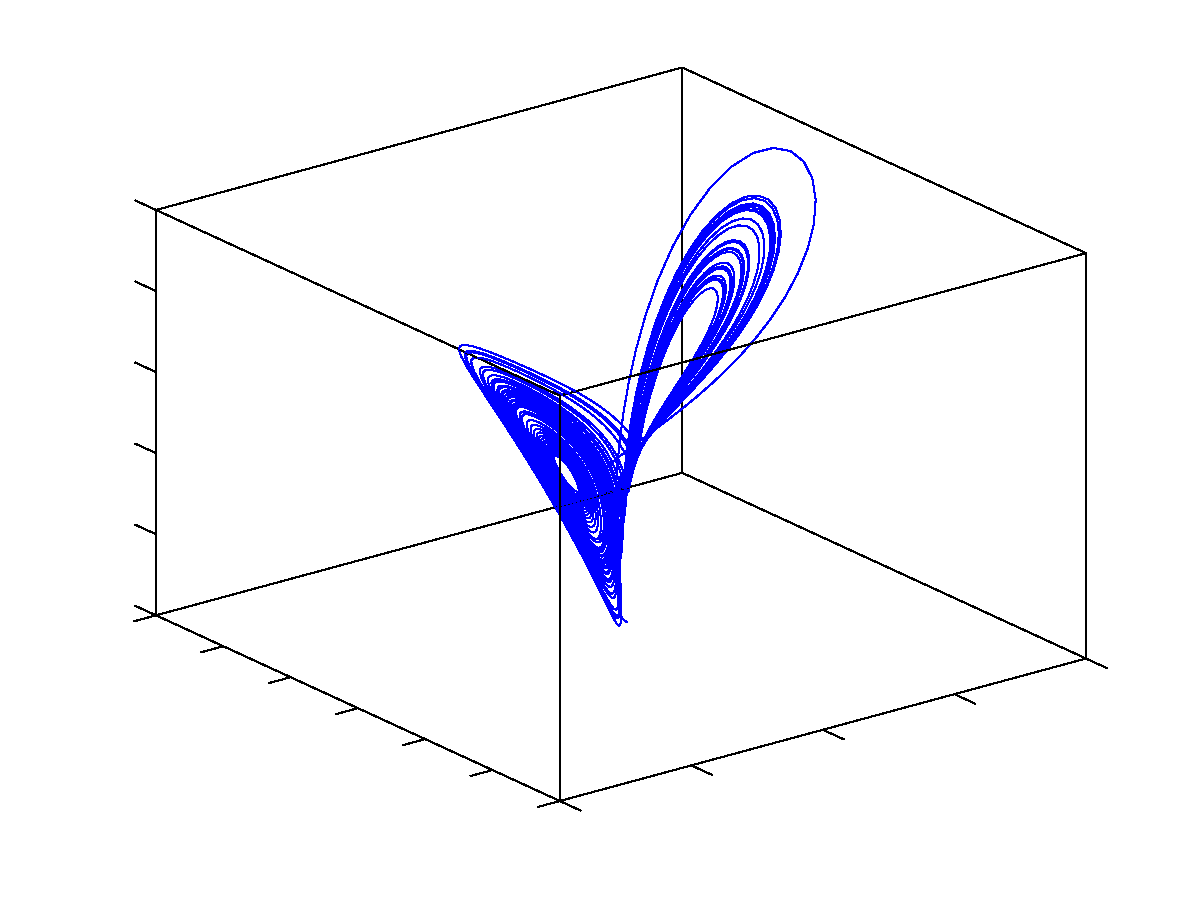
\includegraphics{CurvaLorentz-inc}
\end{picture}%
\begin{picture}(576,432)(0,0)
\fontsize{10}{0}
\selectfont\put(188.51,73.009){\makebox(0,0)[tr]{\textcolor[rgb]{0,0,0}{{-10}}}}
\fontsize{10}{0}
\selectfont\put(156.207,87.8628){\makebox(0,0)[tr]{\textcolor[rgb]{0,0,0}{{0}}}}
\fontsize{10}{0}
\selectfont\put(123.905,102.716){\makebox(0,0)[tr]{\textcolor[rgb]{0,0,0}{{10}}}}
\fontsize{10}{0}
\selectfont\put(91.602,117.57){\makebox(0,0)[tr]{\textcolor[rgb]{0,0,0}{{20}}}}
\fontsize{10}{0}
\selectfont\put(59.2995,132.424){\makebox(0,0)[tr]{\textcolor[rgb]{0,0,0}{{30}}}}
\fontsize{10}{0}
\selectfont\put(220.812,58.1553){\makebox(0,0)[tr]{\textcolor[rgb]{0,0,0}{{-20}}}}
\fontsize{10}{0}
\selectfont\put(60.2059,143.39){\makebox(0,0)[br]{\textcolor[rgb]{0,0,0}{{0}}}}
\fontsize{10}{0}
\selectfont\put(60.2059,182.304){\makebox(0,0)[br]{\textcolor[rgb]{0,0,0}{{10}}}}
\fontsize{10}{0}
\selectfont\put(60.2059,221.219){\makebox(0,0)[br]{\textcolor[rgb]{0,0,0}{{20}}}}
\fontsize{10}{0}
\selectfont\put(60.2059,260.133){\makebox(0,0)[br]{\textcolor[rgb]{0,0,0}{{30}}}}
\fontsize{10}{0}
\selectfont\put(60.2059,299.047){\makebox(0,0)[br]{\textcolor[rgb]{0,0,0}{{40}}}}
\fontsize{10}{0}
\selectfont\put(60.2059,337.962){\makebox(0,0)[br]{\textcolor[rgb]{0,0,0}{{50}}}}
\fontsize{10}{0}
\selectfont\put(298.08,409.6){\makebox(0,0)[b]{\textcolor[rgb]{0,0,0}{{Curva de Lorentz con parámetros $\alpha=10$, $\beta=28$ y $\rho=\frac{8}{3}$}}}}
\fontsize{10}{0}
\selectfont\put(253.115,43.3016){\makebox(0,0)[tr]{\textcolor[rgb]{0,0,0}{{-30}}}}
\fontsize{10}{0}
\selectfont\put(283.369,40.7724){\makebox(0,0)[tl]{\textcolor[rgb]{0,0,0}{{-20}}}}
\fontsize{10}{0}
\selectfont\put(346.515,57.8688){\makebox(0,0)[tl]{\textcolor[rgb]{0,0,0}{{-10}}}}
\fontsize{10}{0}
\selectfont\put(409.662,74.9653){\makebox(0,0)[tl]{\textcolor[rgb]{0,0,0}{{0}}}}
\fontsize{10}{0}
\selectfont\put(472.808,92.0618){\makebox(0,0)[tl]{\textcolor[rgb]{0,0,0}{{10}}}}
\fontsize{10}{0}
\selectfont\put(535.954,109.158){\makebox(0,0)[tl]{\textcolor[rgb]{0,0,0}{{20}}}}
\end{picture}
}
\caption{Atractor de Lorentz}
\label{Lorentz}
\end{figure}

Hacia 1960, el meteorólogo Edward Lorentz se dedicaba a estudiar el comportamiento de la
atmósfera, tratando de encontrar un modelo matemático, un conjunto de ecuaciones, que
permitiera predecir a partir de variables sencillas, mediante simulaciones de ordenador, el
comportamiento de grandes masas de aire, en definitiva, que permitiera hacer predicciones
climatológicas.

Lorentz realizó distintas aproximaciones hasta que consiguió ajustar el modelo a la influencia de tres
variables que expresan como cambian a lo largo del tiempo, la velocidad y la temperatura del aire.
El modelo se concretó en tres ecuaciones matemáticas, bastante simples, conocidas, hoy en día,
como modelo de Lorentz y que mostramos a continuación:
\begin{equation}\left.
\begin{array}{l}
\frac{\partial x}{\partial t}=\alpha \cdot (y-x)\\
\\
\frac{\partial y}{\partial t}=x\cdot(\beta-z)-y\\
\\
\frac{\partial z}{\partial t}=x\cdot y-\rho\cdot z\\
\end{array}\right\},
\end{equation}

donde $(x(t),y(t),z(t))$ representa el estado del sistema en el tiempo y $\alpha, \beta$ y $\rho$ son los parámetros del modelo y presenta condiciones iniciales en tiempo $t_0$ de $(x_0,y_0,z_0)$.
Puedes experimentar como es la Curva de Lorentz variando los parámetros y las condiciones iniciales. Nosotros te vamos a mostrar el caso donde Lorentz descubrió
que pequeñas diferencias en los datos de
partida (algo aparentemente tan simple como utilizar 3 ó 6 decimales) llevaban a grandes diferencias
en las predicciones del modelo. Los valores de los parámetros son $\alpha=10$, $\beta=28$ y $\rho=\frac{8}{3}$ y las condicones iniciales $(1,1,1)$.
La curva de Lorentz presentada para estos parámetros puede ser observada en la Figura \ref{Lorentz}.

El nombre de efecto mariposa viene dado por dos razones. Una de ellas porque la forma de la curva de Lorentz parece sugerir una mariposa y la otra razón es que cuando Lorentz intentó explicar esta idea mediante un ejemplo hipotético. Sugirió que imaginásemos a un meteorólogo que hubiera conseguido hacer una predicción muy exacta del comportamiento de la
atmósfera, mediante cálculos muy precisos y a partir de datos muy exactos. Podría encontrarse una
predicción totalmente errónea por no haber tenido en cuenta el aleteo de una mariposa en el otro
lado del planeta. Ese simple aleteo podría introducir perturbaciones en el sistema que llevaran a la predicción de una tormenta. 

Veamos las proyecciones en diferentes planos en la Figura \ref{proyecciones}.

\begin{figure}[ht!]
\centering \scalebox{0.4}{% Title: glps_renderer figure
% Creator: GL2PS 1.3.8, (C) 1999-2012 C. Geuzaine
% For: Octave
% CreationDate: Thu Nov 13 09:32:19 2014
\setlength{\unitlength}{1pt}
\begin{picture}(0,0)
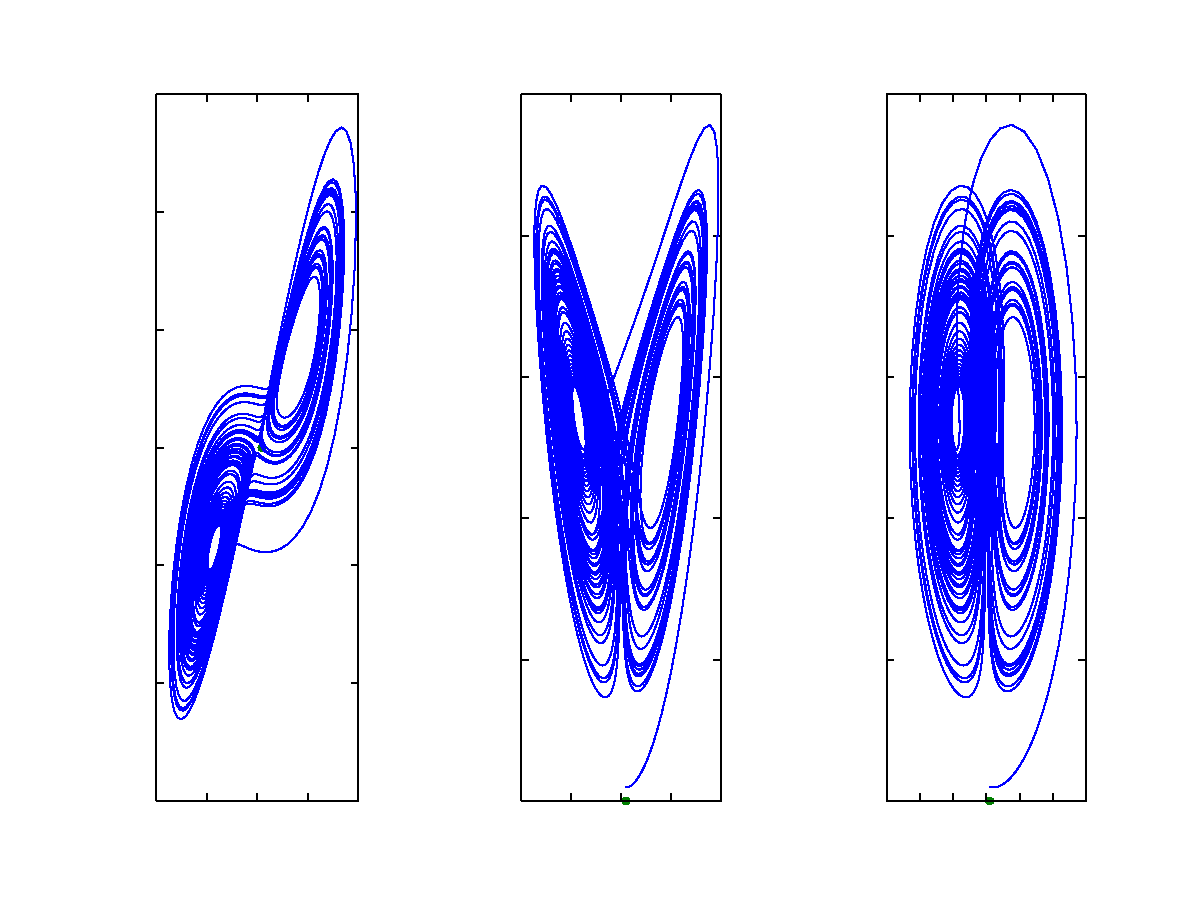
\includegraphics{Proyecciones-inc}
\end{picture}%
\begin{picture}(576,432)(0,0)
\fontsize{10}{0}
\selectfont\put(74.88,42.5167){\makebox(0,0)[t]{\textcolor[rgb]{0,0,0}{{-20}}}}
\fontsize{10}{0}
\selectfont\put(99.1304,42.5167){\makebox(0,0)[t]{\textcolor[rgb]{0,0,0}{{-10}}}}
\fontsize{10}{0}
\selectfont\put(123.381,42.5167){\makebox(0,0)[t]{\textcolor[rgb]{0,0,0}{{0}}}}
\fontsize{10}{0}
\selectfont\put(147.631,42.5167){\makebox(0,0)[t]{\textcolor[rgb]{0,0,0}{{10}}}}
\fontsize{10}{0}
\selectfont\put(171.882,42.5167){\makebox(0,0)[t]{\textcolor[rgb]{0,0,0}{{20}}}}
\fontsize{10}{0}
\selectfont\put(69.8799,47.52){\makebox(0,0)[r]{\textcolor[rgb]{0,0,0}{{-30}}}}
\fontsize{10}{0}
\selectfont\put(69.8799,104.057){\makebox(0,0)[r]{\textcolor[rgb]{0,0,0}{{-20}}}}
\fontsize{10}{0}
\selectfont\put(69.8799,160.594){\makebox(0,0)[r]{\textcolor[rgb]{0,0,0}{{-10}}}}
\fontsize{10}{0}
\selectfont\put(69.8799,217.131){\makebox(0,0)[r]{\textcolor[rgb]{0,0,0}{{0}}}}
\fontsize{10}{0}
\selectfont\put(69.8799,273.669){\makebox(0,0)[r]{\textcolor[rgb]{0,0,0}{{10}}}}
\fontsize{10}{0}
\selectfont\put(69.8799,330.206){\makebox(0,0)[r]{\textcolor[rgb]{0,0,0}{{20}}}}
\fontsize{10}{0}
\selectfont\put(69.8799,386.743){\makebox(0,0)[r]{\textcolor[rgb]{0,0,0}{{30}}}}
\fontsize{10}{0}
\selectfont\put(123.381,396.743){\makebox(0,0)[b]{\textcolor[rgb]{0,0,0}{{Platos}}}}
\fontsize{10}{0}
\selectfont\put(250.24,42.5167){\makebox(0,0)[t]{\textcolor[rgb]{0,0,0}{{-20}}}}
\fontsize{10}{0}
\selectfont\put(274.16,42.5167){\makebox(0,0)[t]{\textcolor[rgb]{0,0,0}{{-10}}}}
\fontsize{10}{0}
\selectfont\put(298.08,42.5167){\makebox(0,0)[t]{\textcolor[rgb]{0,0,0}{{0}}}}
\fontsize{10}{0}
\selectfont\put(322,42.5167){\makebox(0,0)[t]{\textcolor[rgb]{0,0,0}{{10}}}}
\fontsize{10}{0}
\selectfont\put(345.92,42.5167){\makebox(0,0)[t]{\textcolor[rgb]{0,0,0}{{20}}}}
\fontsize{10}{0}
\selectfont\put(245.257,47.52){\makebox(0,0)[r]{\textcolor[rgb]{0,0,0}{{0}}}}
\fontsize{10}{0}
\selectfont\put(245.257,115.365){\makebox(0,0)[r]{\textcolor[rgb]{0,0,0}{{10}}}}
\fontsize{10}{0}
\selectfont\put(245.257,183.209){\makebox(0,0)[r]{\textcolor[rgb]{0,0,0}{{20}}}}
\fontsize{10}{0}
\selectfont\put(245.257,251.054){\makebox(0,0)[r]{\textcolor[rgb]{0,0,0}{{30}}}}
\fontsize{10}{0}
\selectfont\put(245.257,318.898){\makebox(0,0)[r]{\textcolor[rgb]{0,0,0}{{40}}}}
\fontsize{10}{0}
\selectfont\put(245.257,386.743){\makebox(0,0)[r]{\textcolor[rgb]{0,0,0}{{50}}}}
\fontsize{10}{0}
\selectfont\put(298.08,396.743){\makebox(0,0)[b]{\textcolor[rgb]{0,0,0}{{Mariposa}}}}
\fontsize{10}{0}
\selectfont\put(425.6,42.5167){\makebox(0,0)[t]{\textcolor[rgb]{0,0,0}{{-30}}}}
\fontsize{10}{0}
\selectfont\put(441.547,42.5167){\makebox(0,0)[t]{\textcolor[rgb]{0,0,0}{{-20}}}}
\fontsize{10}{0}
\selectfont\put(457.493,42.5167){\makebox(0,0)[t]{\textcolor[rgb]{0,0,0}{{-10}}}}
\fontsize{10}{0}
\selectfont\put(473.44,42.5167){\makebox(0,0)[t]{\textcolor[rgb]{0,0,0}{{0}}}}
\fontsize{10}{0}
\selectfont\put(489.387,42.5167){\makebox(0,0)[t]{\textcolor[rgb]{0,0,0}{{10}}}}
\fontsize{10}{0}
\selectfont\put(505.333,42.5167){\makebox(0,0)[t]{\textcolor[rgb]{0,0,0}{{20}}}}
\fontsize{10}{0}
\selectfont\put(521.28,42.5167){\makebox(0,0)[t]{\textcolor[rgb]{0,0,0}{{30}}}}
\fontsize{10}{0}
\selectfont\put(420.617,47.52){\makebox(0,0)[r]{\textcolor[rgb]{0,0,0}{{0}}}}
\fontsize{10}{0}
\selectfont\put(420.617,115.365){\makebox(0,0)[r]{\textcolor[rgb]{0,0,0}{{10}}}}
\fontsize{10}{0}
\selectfont\put(420.617,183.209){\makebox(0,0)[r]{\textcolor[rgb]{0,0,0}{{20}}}}
\fontsize{10}{0}
\selectfont\put(420.617,251.054){\makebox(0,0)[r]{\textcolor[rgb]{0,0,0}{{30}}}}
\fontsize{10}{0}
\selectfont\put(420.617,318.898){\makebox(0,0)[r]{\textcolor[rgb]{0,0,0}{{40}}}}
\fontsize{10}{0}
\selectfont\put(420.617,386.743){\makebox(0,0)[r]{\textcolor[rgb]{0,0,0}{{50}}}}
\fontsize{10}{0}
\selectfont\put(473.44,396.743){\makebox(0,0)[b]{\textcolor[rgb]{0,0,0}{{Buho}}}}
\end{picture}
}\caption{Proyecciones sobre los planos}\label{proyecciones}
\end{figure}

hay muchas teorías relacionadas a la Teoría del Caos y al comportamiento fractal. Sugerimos te informes de ello porque las teorías no tienen desperdicio. El desafío que te proponemos es que mires los códigos que te hemos pasado de como dibujar la Figura \ref{Lorentz} y varíes los parámetros y las condiciones iniciales y saques tus propias conclusiones.

\begin{mybox}
  \begin{center}\textcolor{blue}{DESAFIO LORENTZ}\end{center}

  Variando en decimales los parámetros $\alpha=10$, $\beta=28$ y $\rho=\frac{8}{3}$ y las condicones iniciales $(1,1,1)$ dibujar como es la curva de Lorentz. ¿Qué observas?
\end{mybox}


\section{Una matriz curiosa}
En esta sección te proponemos que programes la siguiente matriz:
\begin{mybox}
  \begin{center}\textcolor{blue}{DESAFIO MATRIZ CURIOSA}\end{center}
   Dada la secuencia de $n$ enteros $0,1,2,3,4,5,...,n-1$ construir una matriz que cumple que en cada posición es el mínimo de la secuencia dentro de la fila y columna en la que se encuentra según vamos construyéndola.
\end{mybox}

Por ejemplo para $n=8$ la matriz resultante sería la siguiente:
{\tiny $\begin{bmatrix}
0 & 1 & 2 & 3 & 4 & 5 & 6 & 7\\
1 & 0 & 3 & 2 & 5 & 4 & 7 & 6\\
2 & 3 & 0 & 1 & 6 & 7 & 4 & 5\\
3 & 2 & 1 & 0 & 7 & 6 & 5 & 4\\
4 & 5 & 6 & 7 & 0 & 1 & 2 & 3\\
5 & 4 & 7 & 6 & 1 & 0 & 3 & 2\\
6 & 7 & 4 & 5 & 2 & 3 & 0 & 1\\
7 & 6 & 5 & 4 & 3 & 2 & 1 & 0\\
\end{bmatrix}
$}.  Te animamos a que programes construir esta matriz para fualquier
tamaño $n$ y ver si observas algo especial en ella. Te mostramos en la
Figura \ref{ruben} para $n=64$ la estructura de la matriz por
colores. ¿Qué observas? ¿Parece un comportamiento que se repite? ¿Un
comportamiento fractal?
\begin{center}\begin{figure}[ht!]
\centering 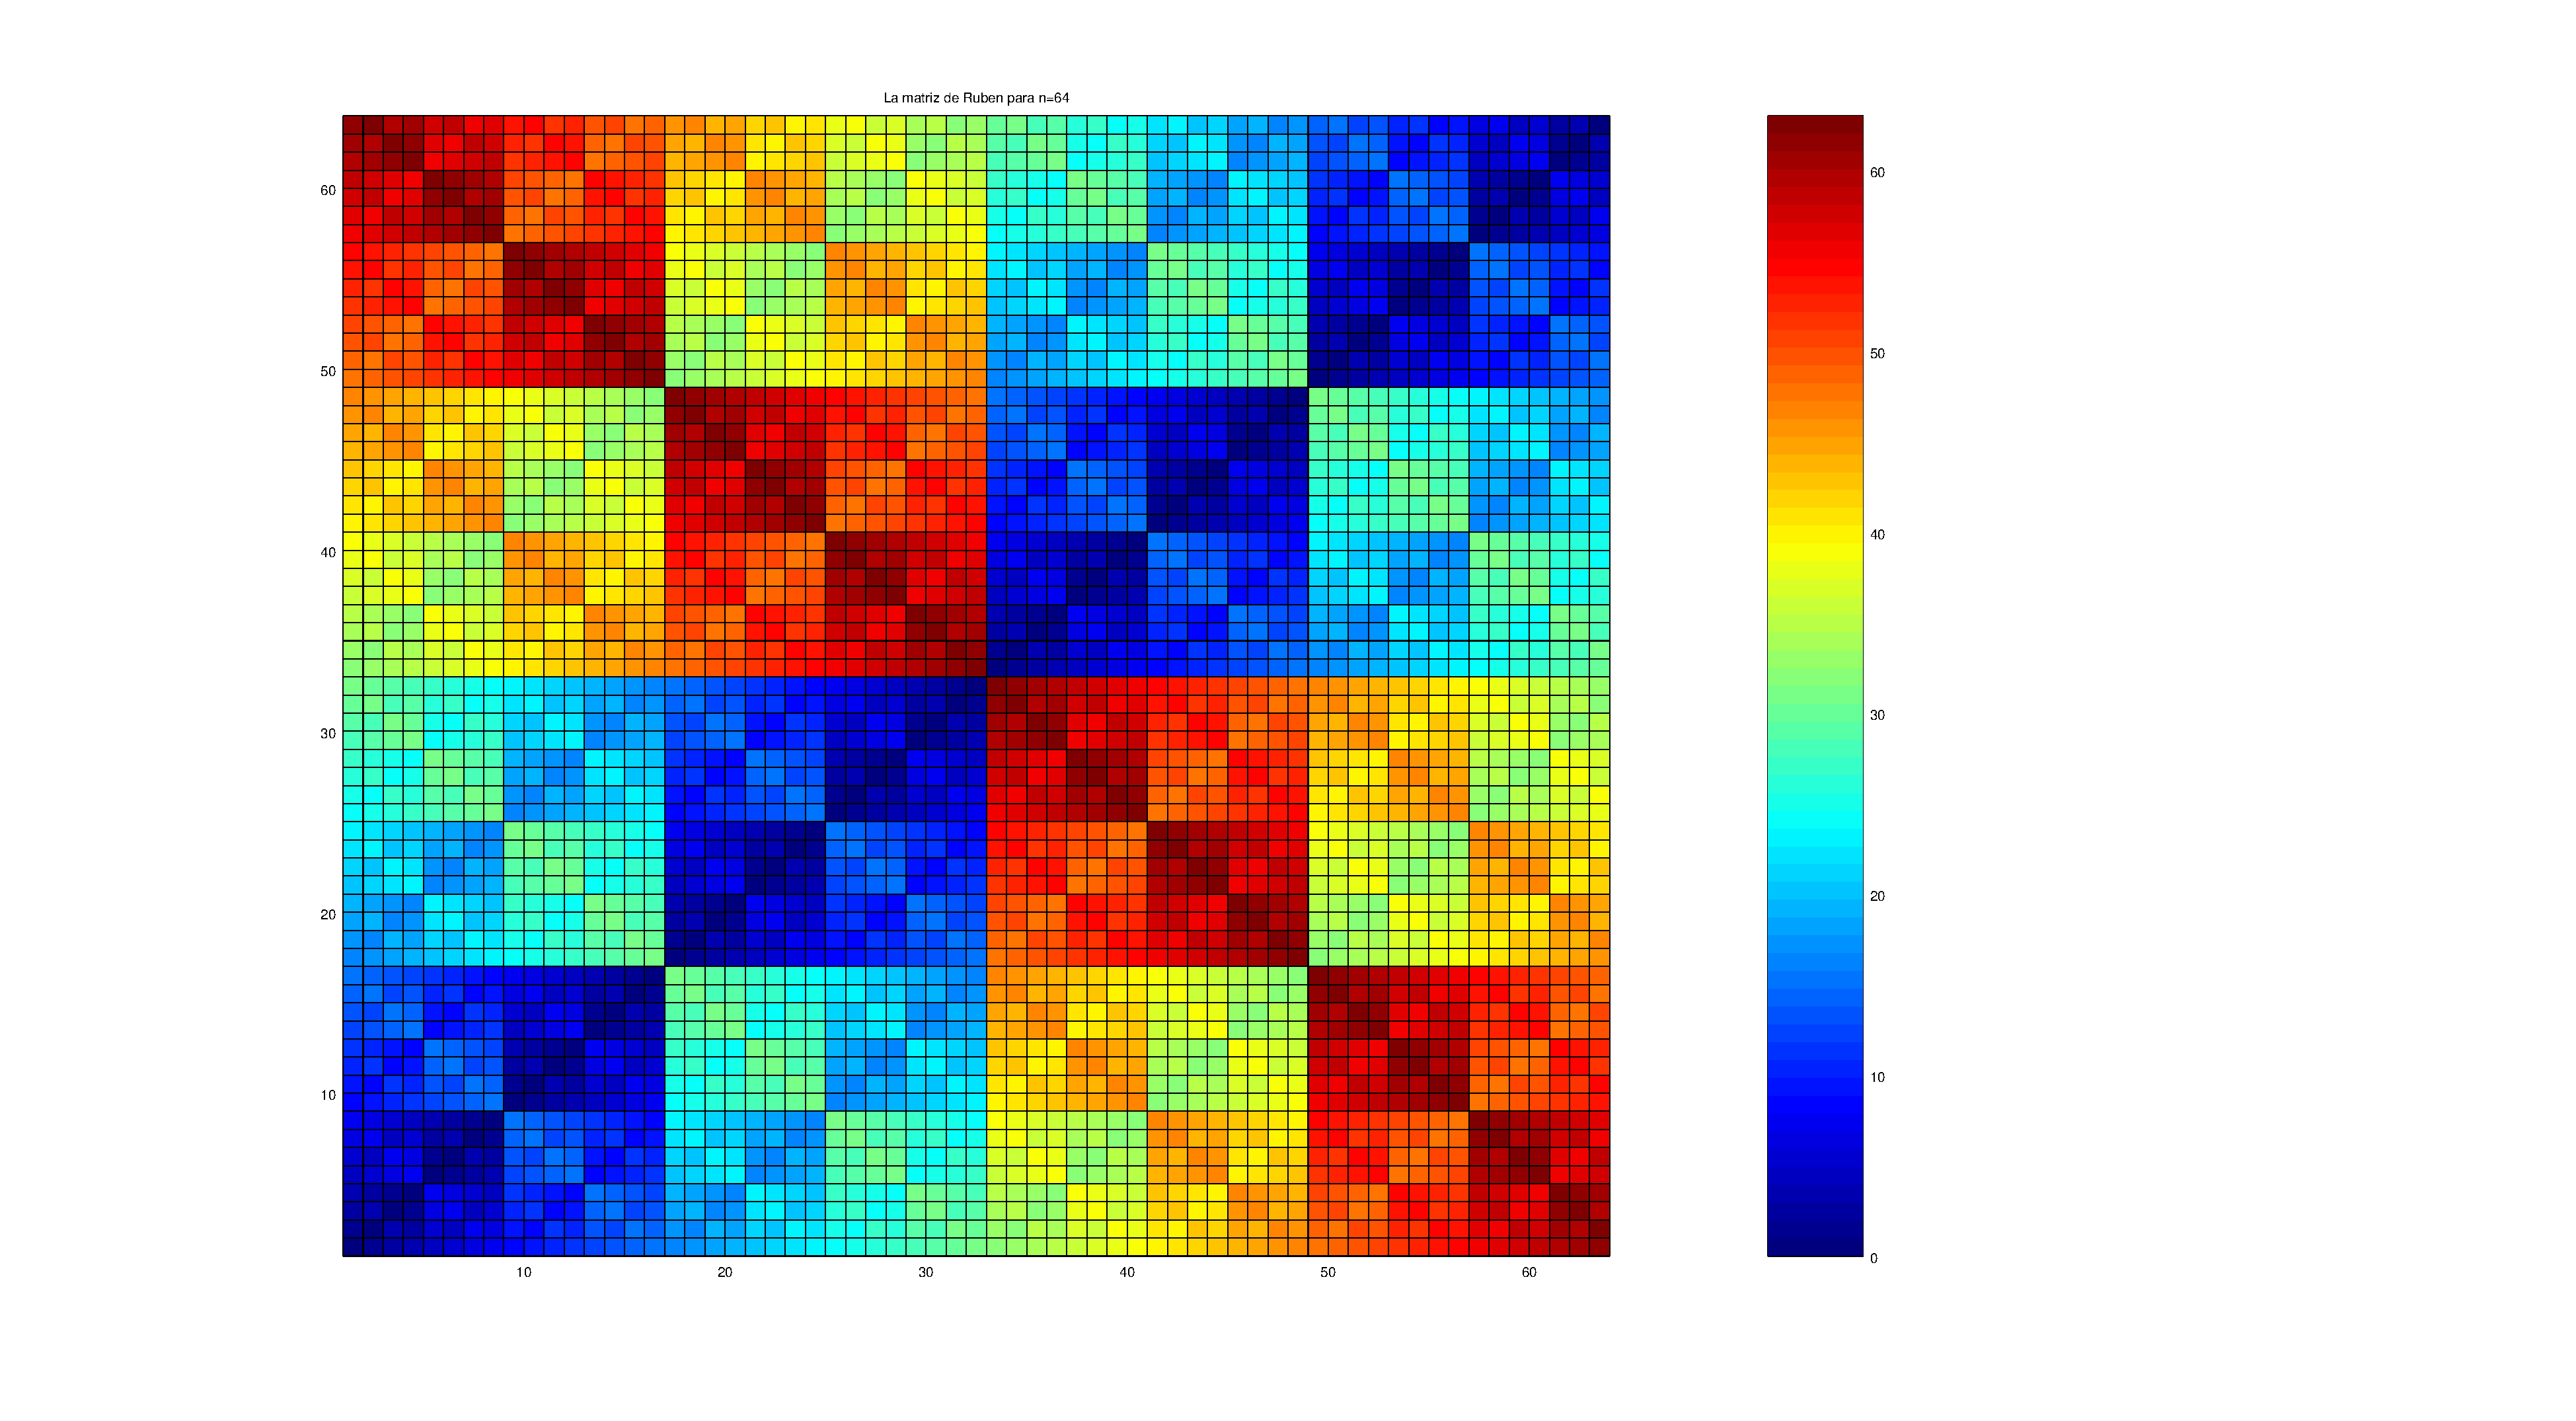
\includegraphics[scale=0.25]{MatrizRuben.eps}\caption{Matriz curiosa para $n=64$.}\label{ruben}
\end{figure}\end{center}

\subsection{Matriz suma binaria}
En esta subsección vamos a animarte a que realices un programa en Octave que programe la siguiente matriz.
\begin{mybox}
 \begin{center}\textcolor{blue}{DESAFIO MATRIZ BINARIA}\end{center}
 Construir una matriz cuadrada de tamaño $n$ cuyas entrada $(i,j)$ es la suma binaria sin llevar de $i-1$ y $j-1$ pasados a numeros binarios. Por ejemplo, la entrada $(6,8)$ se calcula pasando a binario  $6-1=5$ y $8-1=7$ correspondiendose respectivamente  con $11$ y $111$ y la suma en binario sin llevar (Esto es $1+1=0$, $1+0=0+1=1$) es $010$ que se corresponde en sistema decimal con $2$.
\end{mybox}

Te animamos a que la programes y compares con nuestros programas que colgaremos en la sección de códigos de la web de nuestra revista. Te dibujamos a continuación tres mapas de colores de tres matrices de tamaños 4,8 y 16. El comando para ver estos mapas de colores es \emph{pcolor()}. 
\begin{center}
\begin{tabular}{ccc}
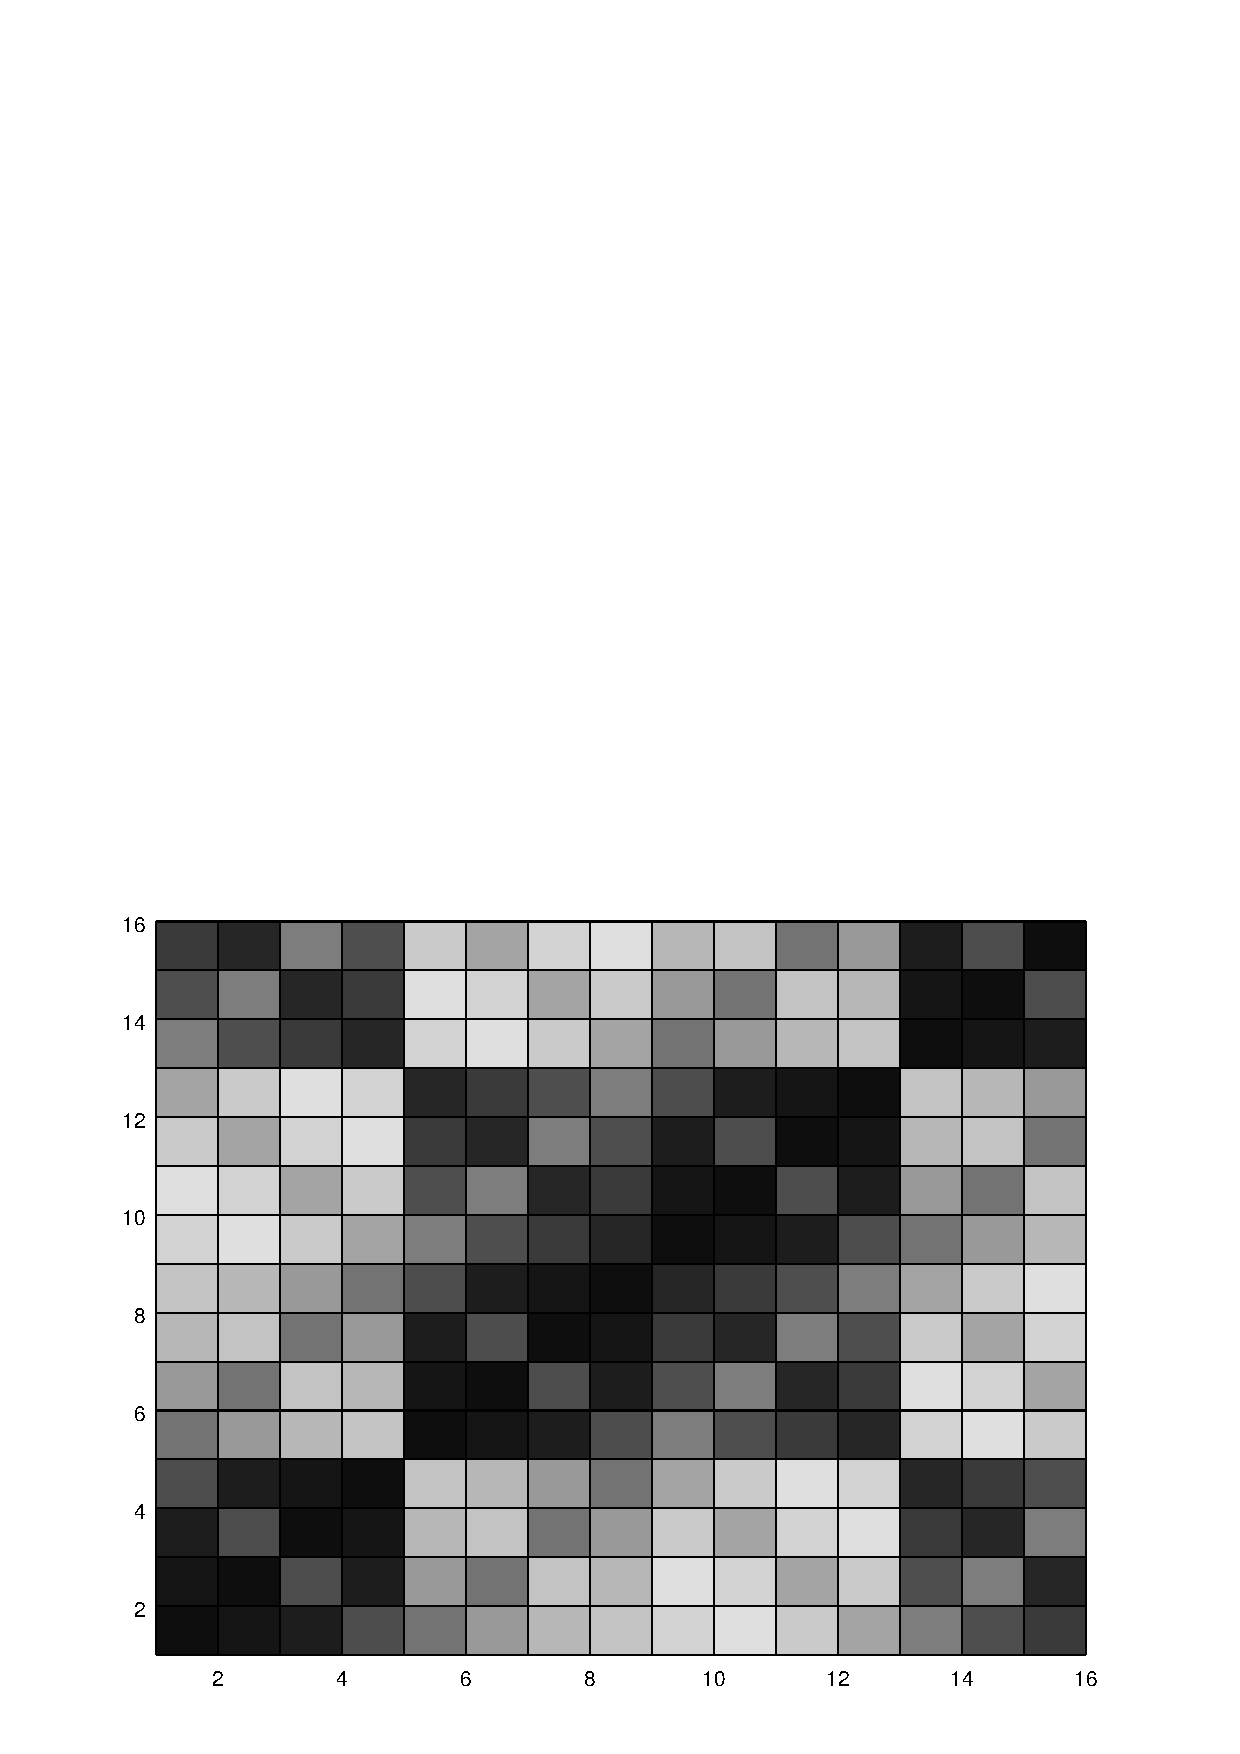
\includegraphics[scale=0.28]{a16.pdf} &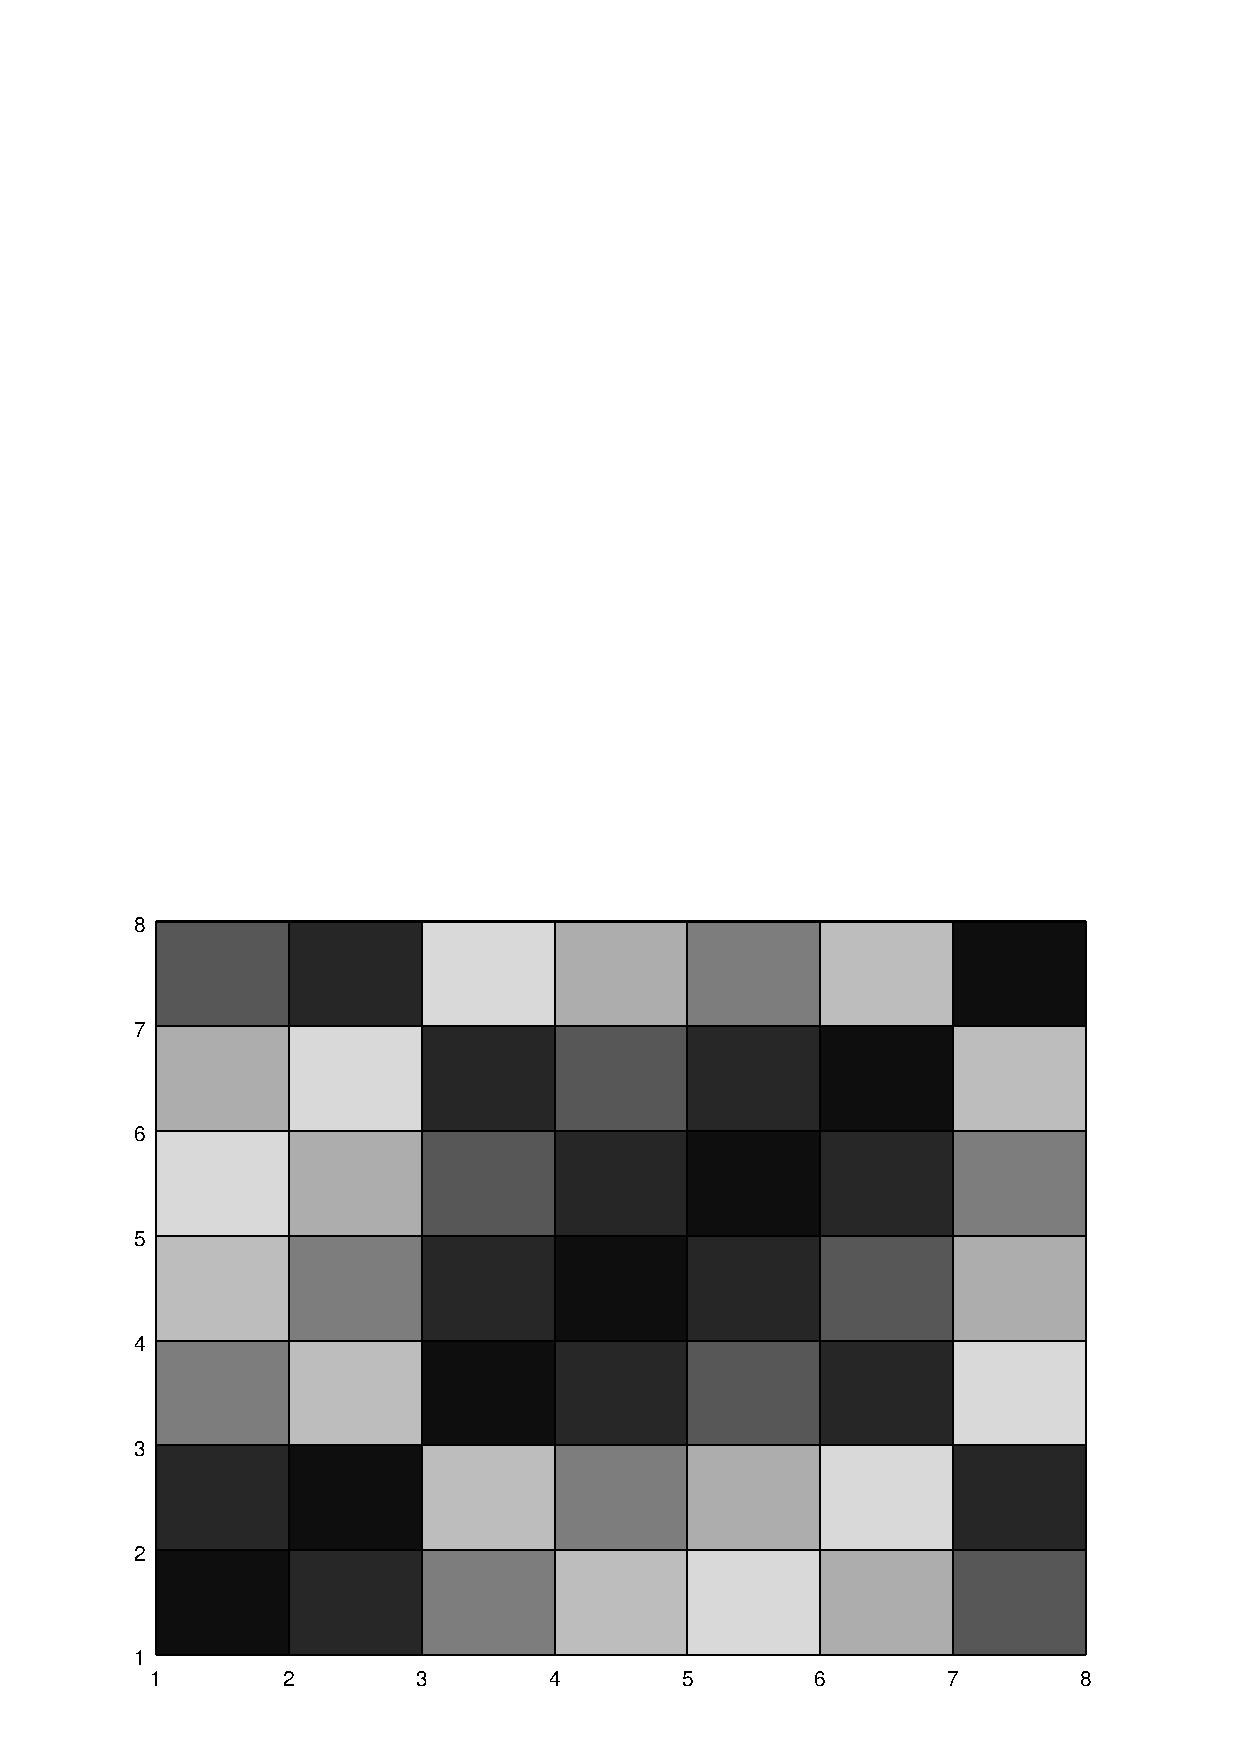
\includegraphics[scale=0.28]{a8.pdf} & \includegraphics[scale=0.28]{a4.pdf}\\
\end{tabular}
\end{center}

¿Te suena algo esta matriz? Parece coincide con la matriz curiosa anterior dada  pero vista desde otro punto de vista y esto nos permite generar estas matrices de forma más eficiente. Matemáticamente esta matriz puede ser estudiada con profundidad y observar preciosas propiedades. Dejamos al lector hacerse adicto a ella.

\section{Arte matemático}
Y para terminar con nuestro curso de \emph{Octave} os proponemos que hagáis vuestro arte con \emph{Octave} y que juguéis con las matemáticas y el dibujar gráficos en 2D y 3D con la herramienta de \emph{Octave}. Os proponemos que mandéis vuestras propuestas por nuestro facebook \url{https://www.facebook.com/revistasolucoes} o al email de la revista \emph{revista@revistasolucoes.com}. Haremos una selección del mejor dibujo \emph{octave soluçoes} y el ganador recibirá un \textcolor{blue}{e-book}(libro electrónico) de regalo. Os damos algunas propuestas en el Cuadro \ref{propos}.

\begin{table}
\begin{center}
\begin{tabular}{c|c}
\includegraphics[scale=0.34]{helado.pdf} & \includegraphics[scale=0.34]{panda.pdf}\\\hline
\includegraphics[scale=0.34]{tren.pdf} &  \includegraphics[scale=0.34]{pinguino.pdf}\\
\end{tabular}\caption{Dibujos hechos con \emph{Octave}}\label{propos}
\end{center}
\end{table}


%\vspace{3cm}
%\noindent
%\includegraphics[width=\textwidth]{pubmm2.png}

\newpage
%%% Local Variables: 
%%% mode: latex
%%% TeX-master: "informaticaeningenieria"
%%% End: 



